\chapter{LITERATURE REVIEW} % TODO: see Howe 1975

Arguably the first notable attempt to design a programming language with an explicit intent of processing sounds and making music was that of \emph{Music I}, created in 1957 by Max Mathews. The language was indented to run on an IBM 704 computer, located at the IBM headquarters in New York City. The programs created there were recorded on digital magnetic tape, then converted to analog at Bell Labs, where Mathews spent most of his career as an electrical engineer. \emph{Music I} was capable of generating a single waveform, namely a triangle, as well as assigning duration, pitch, amplitude, and the same value for decay and release time. \emph{Music II} followed a year later, taking advantage of the much more efficient IBM 7094 to produce up to four independent voices chosen from 16 waveforms. With \emph{Music III}, Mathews introduced in 1960 the concept of a \emph{unit generator}, which consisted of small building blocks of software that allowed composers to make use of the language with a lot less effort and required background. In 1963, \emph{Music IV} introduced the use of macros, which had just been invented, although the programming was still done in assembly language, hence all implementations of the program remained machine-dependent. With the increasing popularity of Fortran, Mathews designed \emph{Music V} with the intent of making it machine-independent, at least in part, since the unit generators' inner loops were still programmed in machine language. The reason for that is the burden these loops imposed on the computer \cite[15-17]{Roads1980}.

\begin{figure}
	\centering
	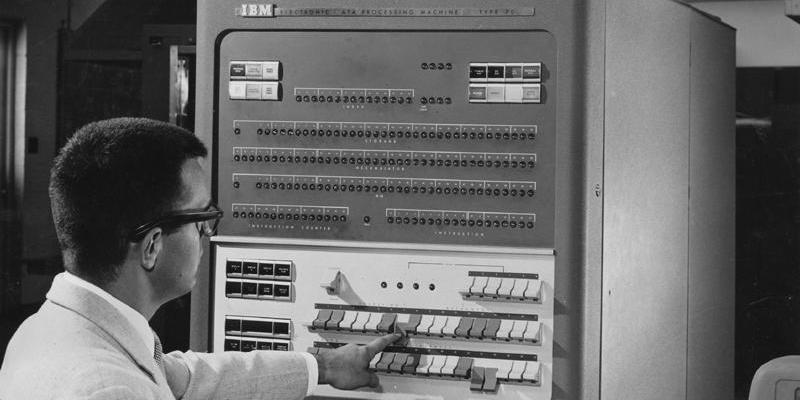
\includegraphics[scale=0.7]{img/IBM704b}
	\caption[The IBM 704 computer.]{The IBM 704 computer.}
\end{figure}

\section{Software Synthesis Languages}

Since Mathews' early work, much progress has been made, and a myriad of new programming languages that support sound processing, as well as domain-specific languages whose sole purpose is to process sounds or musical events, have surfaced. In \cite{Roads1995}, we see an attempt to classify these languages according to the specific aspect of sound processing they perform best. The first broad category described is that of \emph{software synthesis languages}, which compute samples in non-real-time, and are implemented by use of a text editor with a general purpose computer. The \emph{Music N} family of languages consist of software synthesis languages. A characteristic common to all software synthesis languages is that if a toolkit approach to sound synthesis, whereby using the toolkit is straightforward, however customizing it to fulfill particular needs often require knowledge of the programming language in which the toolkit was implemented. This approach provides great flexibility, but at the expense of a much steeper learning curve. Another aspect of software synthesis languages is that they can support an arbitrary number of voices, and the time complexity of the algorithms used only influences the processing time, not the ability to process sound at all, as we see with real-time implementations. As a result of being non-real-time, software synthesis languages usually lack controls that are gestural in nature. Yet, software synthesis languages are capable of processing sounds with a very fine numerical detail, although this usually translates to more detailed, hence verbose code. Software synthesis languages, or non-real-time features of a more general-purpose language, are sometimes required to realize specific musical ideas and sound-processing applications that are impossible to realize in real time \cite[783-787]{Roads1995}.

Within the category of software synthesis languages, we can further classify those that are \emph{unit generator languages}. This is exactly the paradigm originally introduced by \emph{Music III}. In them, we usually have a separation between an orchestra section, and a score section, often given by different files and sub-languages. A unit generator is more often than not a built-in feature of the language. Unit generators can generate or transform buffers of audio data, as well as deal with how the language interacts with the hardware, that is, provide sound input, output, or print statements to the console. Even though one can usually define unit generators in terms of the language itself, the common practice is to define them as part of the language implementation itself. Another characteristic of unit generators is that they are designed to take as input arguments the outputs of other unit generators, thus creating a signal flow. This is implemented by keeping data arrays in memory which are shared by more than one UG procedure by reference. The score sub-language usually consists of a series of statements that call the routines defined by the orchestra sub-language in sequential order, often without making use of control statements. Another important aspect of the score sub-language is that it defines function lookup tables, which are mainly used to generate waveforms and envelopes. When \emph{Music N} languages became machine-independent, function generating routines remained machine-specific for a period of time, due to performance concerns. On the other hand, the orchestra sub-language is where the signal processing routines are defined. These routines are usually called instruments, and basically consist of new scopes of code where built-in functions are dove-tailed, ultimately to a unit generator that outputs sound or a sound file \cite[787-794]{Roads1995}.

The compilation process in \emph{Music N} languages consists usually of three passes. The first pass is a preprocessor, which optimizes the score that will be fed into the subsequent passes. The second pass simply sorts all function and instrument statements into chronological order. The third pass then executes each statement in order, either by filling up tables, or by calling the instrument routines defined in the orchestra. The third pass used to be the performance bottleneck in these language implementations, and during the transition between assembly and Fortran implementations, these were the parts that remained machine-specific. Initially, the output of the third pass consisted of a sound file, but eventually this part of the compilation process was adapted to generate real-time output. At that point, defining specific times for computing function tables became somewhat irrelevant.

In some software synthesis languages, the compiler offers hooks in the first two passes so that users can define their own sound-processing subroutines. In any cases, these extensions to the language were given in an altogether different language. With \emph{Common Lisp Music}, for example, one could define the data structures and control flow in terms of Lisp itself, whereas \emph{MUS10} supported the same features by accepting Algol code. In \emph{Csound}, one can still define control statements in the score using Python. Until \emph{Music IV} and its derivatives, compilation was sample-oriented. As an optimization, \emph{Music V} introduced the idea of computing samples in blocks, where audio samples maintained their time resolution, but control statements could be computed only once per block. Of course, if the block size is one, than we compute control values for each sample, as in the sample-oriented paradigm. Instead of defining a block size, however, one defines a control rate, which is simply the sampling rate times the reciprocal of the block size. Hence a control rate that equals the sampling rate would indicate a block size of one. With \emph{Cmusic}, for instance, we specify the block size directly, a notion that is consistent with the current practice of specifying a vector size in real-time implementations. The idea of determining events in the language that could be computed at different rates required some sort of type declaration. In \emph{Csound}, these are given by naming conventions: variables whose names start with the character `a' are audio-rate variables, `k' means control rate, and `i'-variables values are computed only once per statement. \emph{Csound} also utilizes naming conventions to determine scopes, with the character `g' indicating whether a variable is global \cite[799-802]{Roads1995}.

\section{Real­-Time Synthesis Control Languages}

Some of the very first notable attempts to control the real-time synthesis hardware were made at the \emph{Institut de Recherche et Coordination Acoustique/Musique} in the late seventies. Many of these early attempts made use of programming languages to drive the sound synthesis being carried out by a dedicated DSP. At first, most implementations relied on the concept of a \emph{fixed-function} hardware, which required significantly simpler software implementations, as the latter served mostly to control a circuit that had an immutable design and function. An example of such fixed-function implementations would be an early frequency-modulation synthesized, which contained a dedicated DSP for FM-synthesis, and whose software implementation would only go as far as controlling the parameters thereof. Often, the software would control a chain of interconnected dedicated DSP's, which would in turn produce envelopes, filters, and oscillators. The idea of controlling parameters through software, while delegating all signal processing to hardware, soon expanded beyond the control of synthesis parameters, and into the sequencing of musical events, like in the New England Digital Synclavier. Gradually, these commercial products began to offer the possibility of changing how exactly this components were interconnected, what is called a \emph{variable-function} DSP hardware. Interconnecting these components through software became commonly called \emph{patching}, as an analogy to analog synthesizers. The idea of patching brought more flexibility, but imposed a steeper learning curve to musicians. Eventually, these dedicated DSP's were substituted by general-purpose computers, wherein the entire chain of signal processing would be accomplished via software \cite[802-804]{Roads1995}.

Commonly in a fixed-function implementation there is some sort of front panel with a small LCD, along with buttons and knobs to manage user input. In the case of a keyboard instrument, there is naturally a keyboard to manage this interaction, as well. The purpose of the embedded software is then to communicate user input to an embedded system which contains a microprocessor and does the actual audio signal processing, memory management, and audio input/output. All software is installed in some read-only memory, including the operating system. With the creation of the \emph{Musical Instrument Digital Interface} standard in 1983, which was promptly absorbed my most commercial brands, the issue of controlling sound synthesis hardware transcended the interaction with keys, buttons, and sliders, and became a matter of software programming, as one could easily communicate with dedicated hardware, by means of a serial interface, MIDI messages containing discrete note data, continuous controller messages, discrete program change messages, as well as system­-exclusive messages. As a trend, many MIDI libraries were written at the time for general-purpose programming languages such as APL, Basic, C, Pascal, Hypertalk, Forth, and Lisp. In addition, most descendants of the \emph{Music N} family of languages began to also support MIDI messages as a way to control dedicated hardware \cite[804-805]{Roads1995}.

The implementation of a software application to control variable-function DSP hardware is no mundane task, as it requires knowledge of digital signal processing, in addition to programming in a relatively low level language. Dealing with issues of performance, memory management, let alone the mathematics required to process buffers of audio samples, often imposes an unsurmountable burden to musicians. Many solutions were invented in order to work around this difficulties, including the use of graphic elements and controllers, but ultimately it was the concept of a unit generator, borrowed from software synthesis languages, that most influenced the creation of higher-level abstractions that were more suitable for musicians. This is notably the case of the \emph{4CED} language, which was developed at IRCAM in 1980, and owed greatly to \emph{Music IV} and \emph{Music V}. The resemblance extended as far as to comprise a separate orchestra sub-language for patching unit generators, a score sub-language, and a third command sub-language for controlling effects in real-time, as well as to link both orchestra and score to external input devices such as buttons and potentiometers. The hardware these languages drove was IRCAM's 4C synthesizer. The result of nearly a decade of research at IRCAM culminated in \emph{Max}, a visual programming language that remains to this day one of the most important real-time tools for musicians. \emph{Max}, which will later be discussed in more detail, eventually transcended its hardware DSP and implemented itself in C the sound-generating routines. But that was not until the 2000's, ten years after it became a commercial software application, independent of IRCAM \cite[805-806]{Roads1995}.

\begin{example}
	\cite[809]{Roads1995}
	\emph{Music 1000} is a descendant of the \emph{Music N} family of languages that was designed to drive the Digital Music Systems DMX­1000 signal processing computer, in which we can clearly observe the unit-generator concept in action. In Listing \ref{alg:music1000}, a \lstinline{fnctn} statement assigns to variable \lstinline{func1} an array of 512 samples using a \lstinline{fourier} series of exactly one harmonically-related sine, whose (trivial) sum is \lstinline{normal}-ized. The amplitude of 1000 is then meaningless, but a required argument. In fact, \lstinline{func1} takes a variable number of arguments, where for each harmonic partial, the user specifies a relative amplitude. The block that follows defines an instrument, in which the unit generator \lstinline{oscil} takes as arguments the output of three other unit generators, which are respectively the wavetable previously computed, as well as amplitude and frequency parameters, whose values are in turn captured by two knobs attached to the machine. The knobs produce values between 0 and 1, and the subsequent arguments to \lstinline{kscale} are scaling parameters. Finally, \lstinline{out} is a unit generator that connects the output of \lstinline{oscil} to the digital-to-analog converter.
\end{example}

\begin{lstlisting}[emph={fnctn,instr,kscale,oscil,out,endin,fourier,normal},emphstyle={\textbf},caption={\emph{Music 1000} algorithm that produces a sine wave.},label={alg:music1000}]
fnctn func1, 512, fourier, normal, 1, 1000
instr 1
	kscale amp, knob1, 0, 10000
	kscale freq, knob2, 20, 2000
	oscil x8, #func1, amp, freq
	out x8
endin
\end{lstlisting}

\section{Music Composition Languages}

Between the 1960's and the 1990's, many programming languages were devised to aid music composition. As a noticeable trend, one can define two categories among those languages, namely those that are \emph{score input languages}, and those that are \emph{procedural languages}. The main difference between the two categories is that, in the former, some representation of a musical composition is already at hand, hence score input languages provide a way to encode that information. This could be a score, a MIDI note list, or even some graphical representation of music. In the latter category, the language provides, or helps define procedures that are used to generate musical material, a practice that is often called \emph{algorithmic} music composition. One outstanding characteristic of score input languages is how verbose and complex they can become, depending on the musical material they are trying to represent. This difficulty influenced the devising of many alternatives to textual programming languages, such as the use of scanners in the late 1990's by Neuratron's \emph{PhotoScore}, an implementation which was predicted by composer Milton Babbitt as early as in 1965. Before the advent of MIDI, however, programming languages were indeed the user interface technology of choice, or lack thereof, to design applications meant for analyzing, synthesizing, and printing musical scores. With the widespread adoption of the MIDI standard in the mid-1980's, whereby one can input note events by performing on a MIDI instrument, combined with the advancements in graphical user interfaces of the mid-1990's, the creation and maintenance of score input languages has faced a huge decline. What is even worse, the paradigm of a musical score is itself inadequate for computer music synthesis, in that a score is more often than not a very incomplete representation of a musical piece, often omitting a great deal of information. It is the job of a musical performer to provide that missing information. In this sense, \emph{procedural languages} are much better suited for computer performance, but that comes at the cost of replacing the score paradigm altogether \cite[811-813]{Roads1995}.

In 2018, a few \emph{score input languages} remain, despite the vast predominance of graphical user interfaces as a means to input notes to a score. \emph{MusiXTex} is a surviving example that compiles to \LaTeX, which in turn compiles to PDF documents. It was created in 1991 by Daniel Taupin. The language has such unwieldy syntax, that often a preprocessor is required for more complex scores. One famous such processors is \emph{PMX}, a \emph{Fortran} tool written by Don Simons in the late 1990's. Another was \emph{MPP}, which stands for MusiXTex Preprocessor, created by Han-Wen Nienhuys and Jan Nieuwenhuizen in 1996, and which eventually became \emph{LilyPond}, arguably the most complete surviving score input language today. \emph{LilyPond} has a much simpler syntax than that of \emph{MusiXTex}, however not nearly as simple as \emph{ABC} music notation, a language that much resembles \emph{Musica} and which is traditionally used in music education contexts. A package written by Guido Gonzato is available in \LaTeX which can produce simple scores in \emph{ABC} notation. Its simplicity comes, however, at the expense of incompleteness. Finally, it is worthwhile to mention a music-notation specific standard that has emerged in the mid-2000's, namely the \emph{MusicXML} standard. Heavily influenced by the industry, it was initially meant as an object model to translate scores between commercial applications where the score input method was primarily graphical, and whose underlying implementation was naturally object-oriented. \emph{MusicXML} is extremely verbose, and borderline human-readable. It is, however, very complete, to the point of dictating what features an object-oriented implementation should comprise in order to be aligned with the industry standards. In recent years, many rumors have surfaced to make \emph{MusicXML} an Internet standard, such as that of \emph{Scalable Vector Graphics}, however nothing concrete has been established.

\begin{lstlisting}[caption={\emph{Musica} algorithm that creates a simple melodic line.}]
4'AGAG / 4.A8G2E / 4DDFD / 2ED
\end{lstlisting}

\begin{example}
	\cite[812]{Roads1995}
	\emph{Musica} was developed at the Centro di Sonologia Computazionale in Padua, Italy, and is particularly interesting in its interpreter compiles programs into \emph{Music V} note statements.
	\noindent In the snippet above, all numbers indicate note duration, that is, 4 is a quarter-note, 8 is an eighth-note, and 2 is half-note, with dots indicating dotted durations. The letters indicate pitch, and the apostrophe indicates octave such that '$A = 440$Hz, and ''$A = 880$Hz. Finally, the slash indicates a measure. The code below, on the other hand, shows an example of the very same musical material expressed in \emph{MusiXTex}. One can immediately notice the difference in implementation by the sheer amount of code required to express basically the same symbols.
	\noindent In the code above, many commands, despite verbose, are quite self-explanatory. Some others, however, are not. The \lstinline{\qu} command means a quarter-note with a stem pointing upward, whereas the \lstinline{\Notes} command actually means how notes should be spaced. The more capital letters, the more spacing between the notes, that is, \lstinline{\NOTes} is more spaced out than \lstinline{\NOtes}. Finally, in addition to supporting the same apostrophes as \emph{Musica} for defining octave, \emph{MusiXTex} also supports other letters, as well as capitalizations thereof. In the example above, we have $h = 440$Hz, whereas $a = 220$Hz.
\end{example}

\begin{lstlisting}[caption={\emph{MusiXTex} algorithm whose output is shown in Fig.~\ref{doremi}.}]
\begin{music}
	\generalmeter{\meterfrac44}
	\startextract
	\Notes \qu{h g h g} \en \bar
	\Notes \qup{h} \cu{g} \hu{e} \en \bar
	\Notes \qu{d d f d} \en \bar
	\Notes \hu{e d} \en
	\endextract
\end{music}
\end{lstlisting}

\begin{figure}
	\caption{Typesetting music with \emph{MusiXTex}.}
	\label{doremi}
	\centering
	\begin{music}
		\generalmeter{\meterfrac44}
		\startextract
		\Notes \qu{h g h g} \en \bar
		\Notes \qup{h} \cu{g} \hu{e} \en \bar
		\Notes \qu{d d f d} \en \bar
		\Notes \hu{e d} \en
		\endextract
	\end{music}
\end{figure}

One of the greatest contributions of \emph{procedural composition languages} to the field of music composition is arguably the concept of algorithmic composition, in particular when the realization of the musical algorithm is not restricted to human performers. In such circumstances, the composer is capable of exploring the full extent of musical ideas a computer can reproduce. Naturally, the composer must often trade off the ability to represent those ideas via a score, in which case the algorithm itself becomes the representation. If, on one hand, reading music from an algorithm is somewhat unfamiliar to most musicians, the representation is nonetheless formal, concise, and consistent. Furthermore, it lends itself to be analyzable a much larger apparatus of analytical techniques and visualization tools, hence is equally beneficial a representation to music theorists. A machine is capable of representing all sorts of timbres, metrics, and tunings that humans cannot, but it needs to be told exactly what to do. Unlike a human performer, who interprets the composer's intents, a purely electro-acoustic algorithmic composition must address a human audience without relying on a middle-man. Hence the programming language of choice becomes an invaluable tool for the composer. In addition to all that, another important aspect of algorithmic composition is how it is capable of transforming the decision-making process of a composer. Instead of making firm choices at the onset of a musical idea, a composer can \emph{prototype} many possible outcomes of that idea before deciding. One example is assigning random numbers to certain parameters, this postponing the decision making until more structure has been added to the composition. In fact, this postponing may be final, thus an algorithmic composition may be situated within a whole spectrum of determinism. A fully stochastic piece fixes no parameter, as opposed to a fully deterministic composition. Some of the notable techniques of electro-acoustic music composition also include spatialization, where the emission of sounds through speakers positioned at specific spatial locations constitutes a major musical dimension in a composition; spectralism, where the spectral content of sounds are manipulated by an algorithm; processing sound sources in real time, very often capturing a live performance on stage; and sonification of data nor originally conceived as sound \cite[813]{Roads1995}.

\section{Libraries}

Many domain-specific languages that deal with sound synthesis, processing, and music composition are \emph{extensible} in the sense that they provide a hook for code written in the implementation language to be executed in the context of the DSL. This feature can render a DLS a lot more flexible, at the expense of annulling the very purpose of the DSL, which can be a good trade-off if the latter's implementation is incomplete. An early example would be \emph{Music V}, which could accept user-written subroutines in \emph{Fortran}. \emph{Music 4C} had its instruments written in \emph{C}, and \emph{Cscore} was a \emph{C}-embedding of \emph{Cmusic}. Other examples are \emph{MPL}, which could accept routines written in \emph{APL}, and \emph{Pla}, whose first version was embedded in \emph{Sail}, and whose second version was embedded in \emph{Lisp}. In the particular case of \emph{Lisp}, embeddings include \emph{MIDI-LISP}, \emph{FORMES}, \emph{Esquisse}, \emph{Lisp Kernel}, \emph{Common Music}, \emph{Symbolic Composer}, \emph{Flavors Band}, and \emph{Canon}. \emph{Music Kit} was embedded in the object-oriented \emph{Objective-C} \cite[814]{Roads1995}.

Besides domain-specific languages, a variety of libraries exist for general-purpose programming languages that also deal with aspects of sound synthesis, processing, and music composition. In languages like \emph{Haskell}, these libraries may carry such syntactical weight, with so many specifically-defined symbols, that they do in fact resemble more a DSL that a library, even though such terming would not be technically correct.